\documentclass{article}
%\usepackage{fullpage}
%\usepackage{fullpage}
\usepackage{amsmath}
\usepackage{tikz}
\usepackage{latexsym}
\usepackage{amssymb,amsfonts}
\usepackage{graphicx}
\usepackage{array}
\usepackage{graphics}
\usepackage{wrapfig}
\usepackage{multirow}
\usepackage[margin=.75in]{geometry}

\newcommand{\fillinblank}{ \line(1,0){100} }

\setlength{\parindent}{0.3in}
\setlength{\parskip}{0.1in}

\pagenumbering{gobble}

\begin{document}
\begin{flushleft}
\begin{tabular}{l c r}
 \begin{tabular}{l}
   {\Huge MaPP-Callenge 2021}\\
   {\Huge Reptile Puzzle }\\
   {\Large (Draft)}
   \end{tabular}
    \begin{tabular}{c}
   \hspace{1in}
   \end{tabular}
   
\end{tabular}\begin{tabular}{r}
     \includegraphics[width=2in]{mapp-square.pdf}
 \end{tabular}
   

\thispagestyle{empty}

\noindent\hrulefill
\phantom{.}\vspace{.15in}

The Sphinx is a famous shape that resembles the Great Sphinx at Giza. More interesting is that it can be broken into smaller versions of itself with nothing left as shown in the two images below. (some nondescript way of describing it so they can't search repeated tiling)

\begin{center}
\begin{tabular}{c c c}
\includegraphics[width=2in]{Sphinx4.pdf} &  \hspace{1in} & \includegraphics[width=2in]{Sphinx9.pdf}
\end{tabular}
\end{center}

Use the images from the player book to decode a message by determining how many pieces each shape can be broken into using smaller versions of itself in the same fashion we have decoded the letter ``B'' from the Sphinx below.

\begin{center}
\includegraphics[width=2in]{Sphinx.pdf}

A \hspace{0.5in} B \hspace{0.5in} C \\
4 \hspace{0.54in} 7 \hspace{0.54in} 9

\end{center}

\newpage

\begin{center}
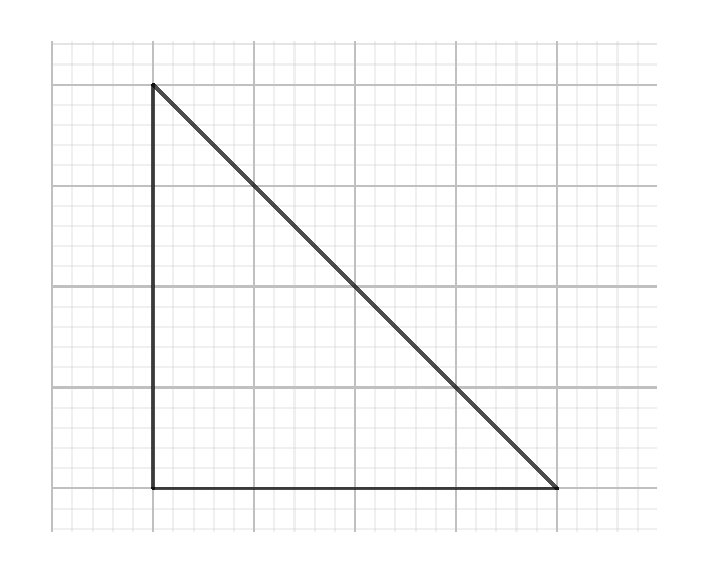
\includegraphics[width=2in]{IsoRightTriangle.pdf}

F \hspace{0.5in} A \hspace{0.5in} C  \hspace{0.5in} T\\
4 \hspace{0.54in} 6 \hspace{0.54in} 8 \hspace{0.54in} 16 

\end{center}

\begin{center}
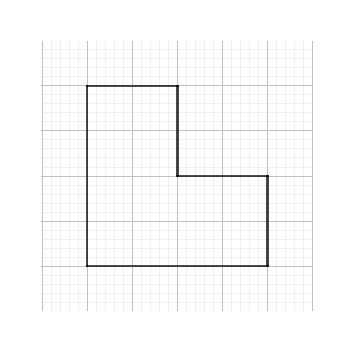
\includegraphics[width=2in]{L-Shape.pdf}

P \hspace{0.5in} L \hspace{0.5in}  A \hspace{0.5in} Y\\
4 \hspace{0.54in} 8 \hspace{0.54in} 9 \hspace{0.54in} 16

\end{center}

\begin{center}
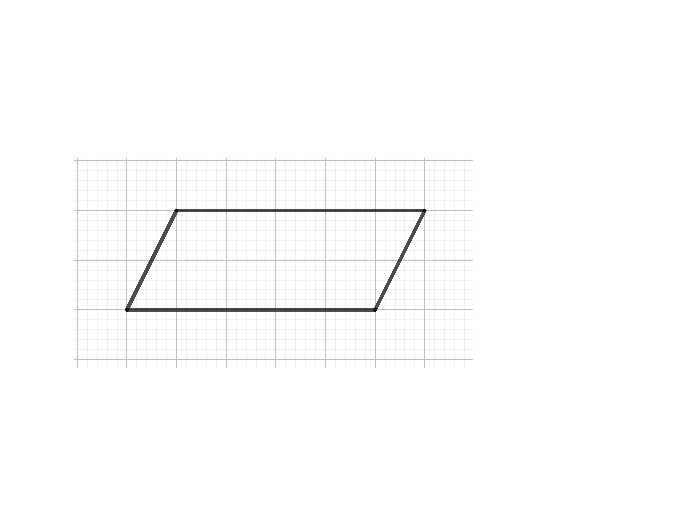
\includegraphics[width=2in]{Parallelogram.pdf}

A \hspace{0.5in} N \hspace{0.5in} T \hspace{0.5in} I \\
5 \hspace{0.52in} 16 \hspace{0.52in} 20 \hspace{0.52in} 21

\end{center}

\begin{center}
\includegraphics[width=2in]{IsoTrap.pdf}

C \hspace{0.5in} L \hspace{0.5in} U \hspace{0.5in} E\\
8 \hspace{0.54in} 9 \hspace{0.54in} 16 \hspace{0.54in} 36

\end{center}

\begin{center}
\includegraphics[width=2in]{1-2RightTri.pdf}

O \hspace{0.5in} P \hspace{0.5in} U \hspace{0.5in} S\\
3 \hspace{0.54in} 4 \hspace{0.54in} 5 \hspace{0.54in} 16

\end{center}


\begin{center}
\includegraphics[width=2in]{30-60-90Tri.pdf}

C \hspace{0.5in} A \hspace{0.5in} R \hspace{0.5in} E \\
3 \hspace{0.54in} 4 \hspace{0.54in} 5 \hspace{0.54in} 16

\end{center}

\begin{center}
\includegraphics[width=2in]{fish.pdf}

N \hspace{0.5in} E \hspace{0.5in} X \hspace{0.5in} T\\
3 \hspace{0.5in} 9 \hspace{0.52in} 81 \hspace{0.52in} 729

\end{center}
\end{flushleft}
\end{document}